We next consider the application of group lasso and grOWL to the discovery of similarity structure in neural responses measured by fMRI across the whole brain while participants perform a cognitive task. In network-based approaches to cognitive neuroscience, mental representations are thought to be encoded as distributed patterns of activation over large neural populations, with different populations encoding different kinds of representational structure and communicating this structure to other network components. As one well-known example, the "triangle" model of reading proposes that words with similar spellings are encoded with similar patterns of activation across some neural population (e.g. activation patterns for DOT will be similar to DOG but not YACHT or POINT); similarity of meaning is encoded with similar patterns of activation across a different population (e.g. patterns for DOT will be similar to POINT but not DOG or YACHT); and similarity of word sound is encoded with patterns of activation across a third population (e.g. pattern for DOT will be similar to YACHT but not DOG or POINT). These different populations are functionally and anatomically connected within a broader network, with separate pathways encoding mappings between spelling, sound, and meaning (Figure XXA). Likewise, network models of visual recognition typically posit different neural populations for encoding visual similarity versus object category and the mappings between these; models of object-directed action propose separate populations for encoding perceptual versus praxic structure and their mappings; models of language comprehension and production propose different systems for encoding semantic versus syntactic structure; and so on.

%There has recently developed considerable interest in testing such models directly using data from functional brain imaging techniques such as fMRI. The best-known approach in this vein has been representational similarity analysis (RSA): across all voxels within a pre-specified cortical region of interest, researchers measure the neural response evoked by each of a large set of stimuli. The distances between vectors of evoked responses are computed for all stimulus pairs, and the resulting neural dissimilarity matrix is correlated with a target matrix that expresses psychophysical distances of interest amongst the stimuli. Such a matrix might contain, for instance, human judgments of perceptual similarity between the stimulus items. Wherever the correlation between the neural and psychophysical distance matrices are reliably non-zero, the corresponding cortical region can be viewed as locally encoding the target similarity structure. This approach to finding structure in brain imaging data has had a broad and deep impact on cognitive neuroscience. 

This general view suggests one way in which the similarity-encoding methods we have considered can be used to discover neural systems that jointly encode a particular kind of representational structure. As with the well-known searchlight representational similarity analysis (\cite{RSA}, \cite{similarity}), we begin with a measurement of the $n \times n $ similarities existing amongst a set of $n$ items in some cognitive domain.  Using fMRI, we measure the neural responses evoked by each item at the scale of single voxels (3mm cubes), and treat these $d$ voxels as features of the $n$ items. We then compute a rank-$r$ approximation of the target similarity matrix $\bS = \bY \bY^T$, and use this as the target $\bY \in \R^{n \times r} $ matrix for a sparse-regression analysis of the $n \times d$ matrix of fMRI responses , $\bX$,  evoked by each item across the whole cortex. The model is then fit to optimize the object functions specified in (\ref{eqn.grouplasso}) for group lasso and (\ref{eqn:L1}) for grOWL. The best regularization parameter is selected through cross-validation, and a final model is fit with that parameter and used to predict the similarities existing amongst a set of items in an independent hold-out set. Model predictions are compared to expected results expected from a null hypothesis that no features encode the target similarity structure. If predictions are more accurate than expected from random data, this provides evidence that the model has discovered voxel subsets that jointly encode some of the target similarity structure. Moreover, because the model is constrained to be sparse, most voxels will receive coefficients of zero, and the presence of non-zero coefficients can be taken as evidence that the corresponding voxel encodes information important to representing the target similarity structure.

The current experiment serves as a proof-of-concept with the aim of answering three questions. First, does either approach work, in the sense of generating above-chance predictions of the similarities existing amongst a set of stimuli given the neural responses they generate across the whole brain? Second, does one approach work better than the other in generating such predictions? Third, does the approach generate solutions that are consistent with what is known about representation of information in the brain?

To answer these questions, we applied the approach to discover voxels that work to encode the visual similarities existing amongst a set of line drawings of common objects. We chose this task and dataset because (a) there exist well-understood methods for objectively measuring the degree of visual similarity amongst such items \cite{antani02} and (b) it is well known that visual similarity is encoded by neural responses in occipital and posterior temporal cortices.

\subsection{fMRI dataset} The data were collected as part of a larger study from 23 participants at the University of Manchester who were compensated for their time. Each participant viewed a series of line drawings depicting common objects while their brains were scanned with fMRI. The line drawings included 37 items, each repeated 4 times for a total of 148 unique stimulus events. At each trial participants pressed a button to indicate whether the item could fit in a ``wheely bin'' (a form of trash can common in the UK).
Scans were collected in a sparse event-related design and underwent standard pre-processing to align functional images to the anatomy and to remove movement and scanner artifact and temporal drift. Responses to each stimulus event were estimated at each voxel using a deconvolution procedure with a standard HRF kernel. For each participant a cortical surface mask was generated based on T1-weighted anatomical images, and functional data were filtered to exclude non-cortical voxels.Voxels with estimated responses more than 5 standard deviations from the mean response across voxels were excluded from the analysis. 10k-15k voxels were selected for each participant, and neural responses across all voxels for each of 148 stimulus events were entered into the analysis. The mean response across the 4 repeated observations of each item were taken to give 37 item responses for each participant. Each column corresponding to a voxel was normalized to be of standard deviation equal to one and a column of ones was added.

\subsubsection*{Target similarities}
 Each stimulus was a bitmap of a black-and-white line drawing. We took pairwise Chamfer distance as a proxy for inter-item visual dissimilarities. r = 3 is the smallest value to attain $\|\bS - \bY\bY^T\|_F \leq 0.2$. This $37 \times 3$ matrix $\bY$ was used as the target matrix for the analysis.

\subsubsection*{Model fitting}
For each participant, training data were divided into 9 subsets containing 4-5 stimulus events each. One subset was selected as a final hold-out set. Models were then fit at each of 10 increasing values of $\lambda$ using 8-fold cross validation. At each fold we assessed the model using the Frobenius norm of the difference between the target $\bY$ entries and the predicted $\hY = \bX\widehat{\bB}$ entries for hold-out items (henceforth the model error). We selected the $\lambda$ with the lowest mean error for each subject subjects, then fit a full model for each subject at this value and assessed it against the final hold-out set, considering the model error on hold-out items. We repeat this process for 9 different final hold-out sets.

\subsection{Results}
%The model cross-validation error at each value of $\lambda$, for both group lasso and grOWL are recorded and the $\lambda$ corresponding to the minimum error  is recorded. %Note that, with no signal in the data, the expected error is 1. The curves show a U-shape with a minimum at XX, and are clearly less than 1. Thus both approaches appear to be generating better predictions for hold-out items than would be expected from random data. 

Figure \ref{fig.error}(a) shows performance on the final hold-out sets for each participant and each method, considering error between predicted ($\bY_z$) and actual dissimilarities ($\bY$). Both approaches show significantly non-random prediction. As in our simulations, the grOWL-|| shows somewhat better performance (lower error, higher correlation) overall all methods have comparable performance in terms of prediction error.

Figure \ref{fig.error}(b) shows the locations of selected voxels (i.e., those with non-zero coefficients) across all 23 participants, projected into a common anatomical space with 2mm full-width-half-max spatial smoothing and projected onto a model of the cortical surface. Left column shows the voxels selected for \textit{at least one} cross-validation run, center column shows the voxels selected for \textit{at least five} (out of nine) cross-validation runs and right column shows the voxels selected for \textit{all} the nine cross-validation runs. As seen in the maps, both methods pick voxels prominently in the occipital and posterior temporal cortices and grOWL-II picks consistently more voxels than group lasso.

Finally, Figure \ref{fig.NW} shows the....

\begin{figure*}[!t]
\centering
\subfloat[]{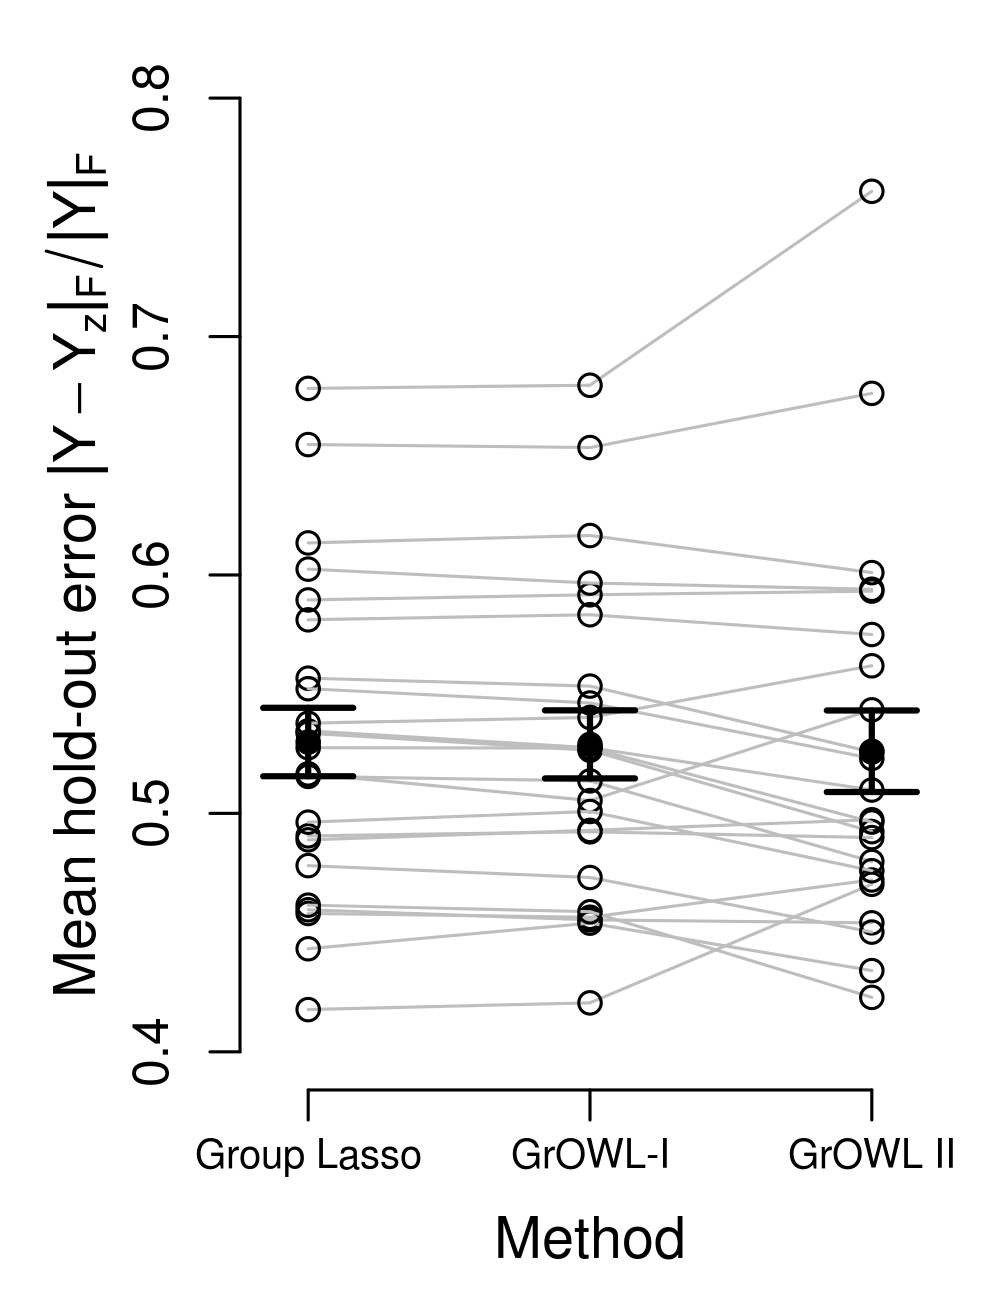
\includegraphics[width=0.3\textwidth]{Final_Error_Visual.png}
\label{fig_first_case}}
\hfil
\subfloat[]{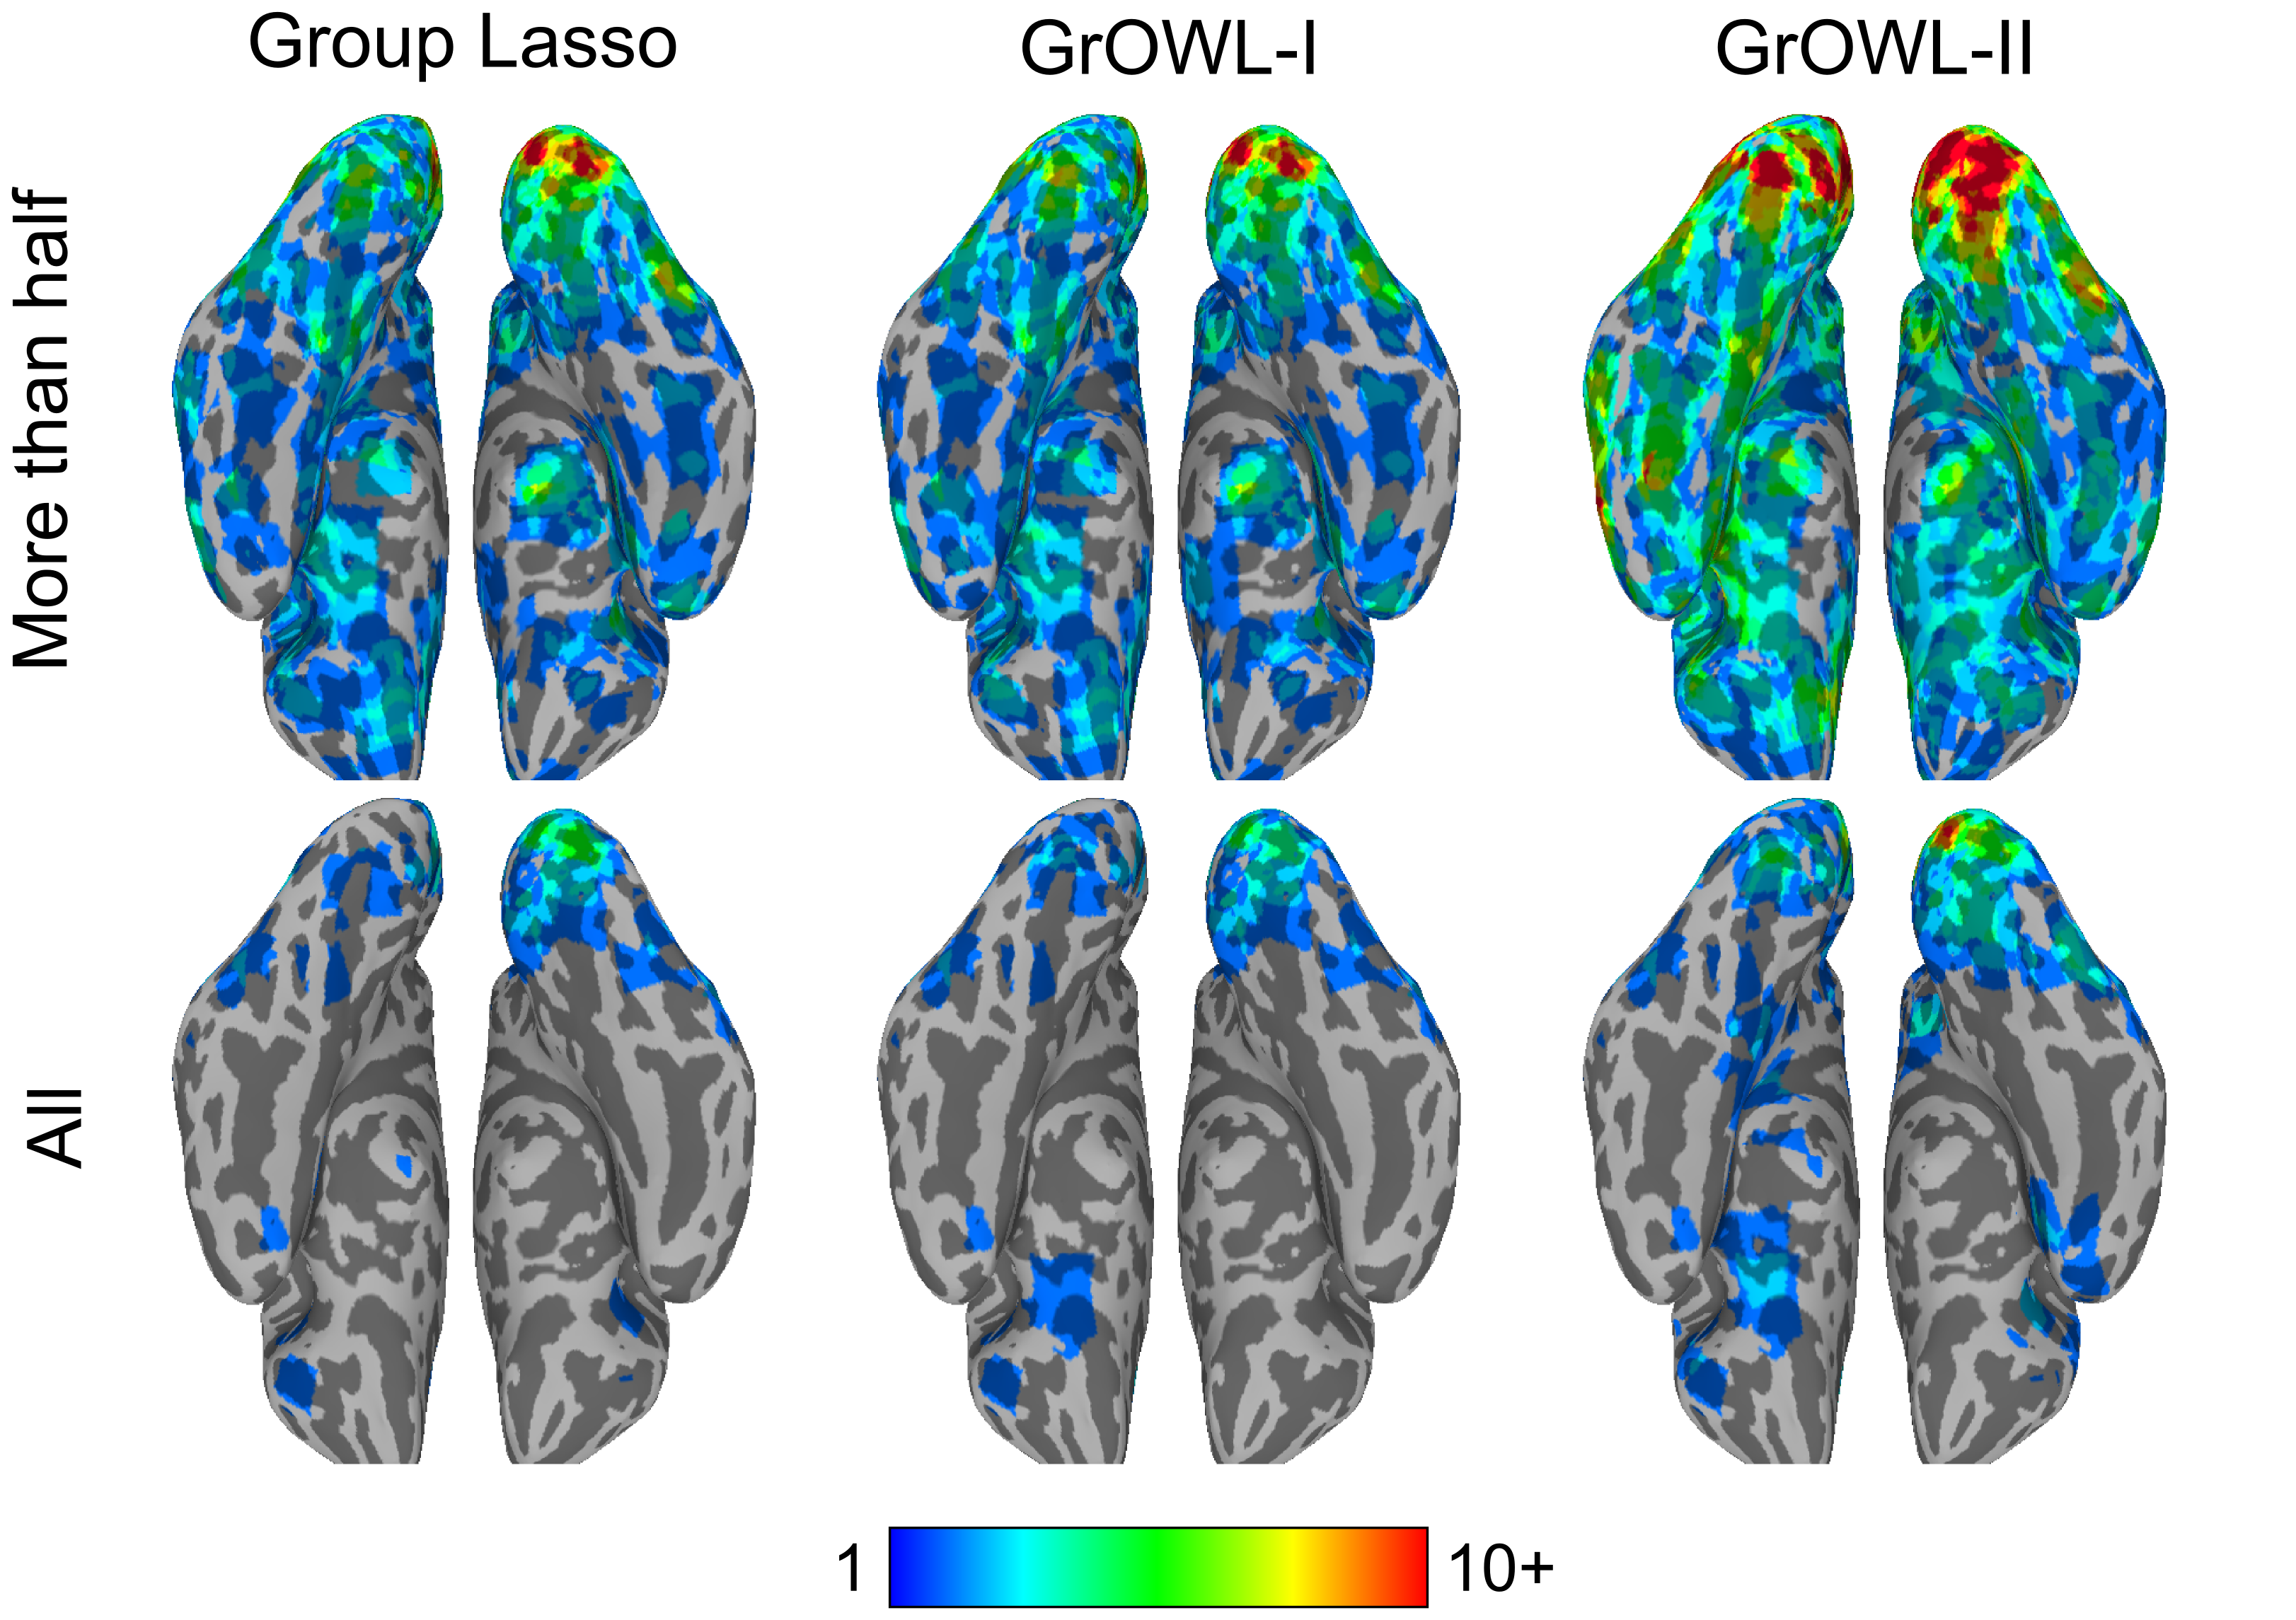
\includegraphics[width=0.6\textwidth]{brain_final.png}
\label{fig_second_case}}
\caption{Panel (a) shows mean hold-out prediction error for group lasso and grOWLs for 23 subjects. Panel (b) shows surface maps corresponding to group lasso (top), grOWL-I (middle) and grOWL-II (bottom) showing the voxels selected for \textit{at least one}, \textit{at least five} and \textit{all nine} cross-validations in the left, center and right columns respectively. The heat map shows the number of subjects for which those voxels were picked. Blue is the least (1 subject) and red is the most (17 subjects).}
\label{fig.error}
\end{figure*}

\begin{figure}[!t]
\centering
\includegraphics[width=0.48\textwidth]{NW.png}%
\caption{Network plots.}
\label{fig.NW}
\end{figure}


\iffalse
\begin{figure*}[!t]
\centering
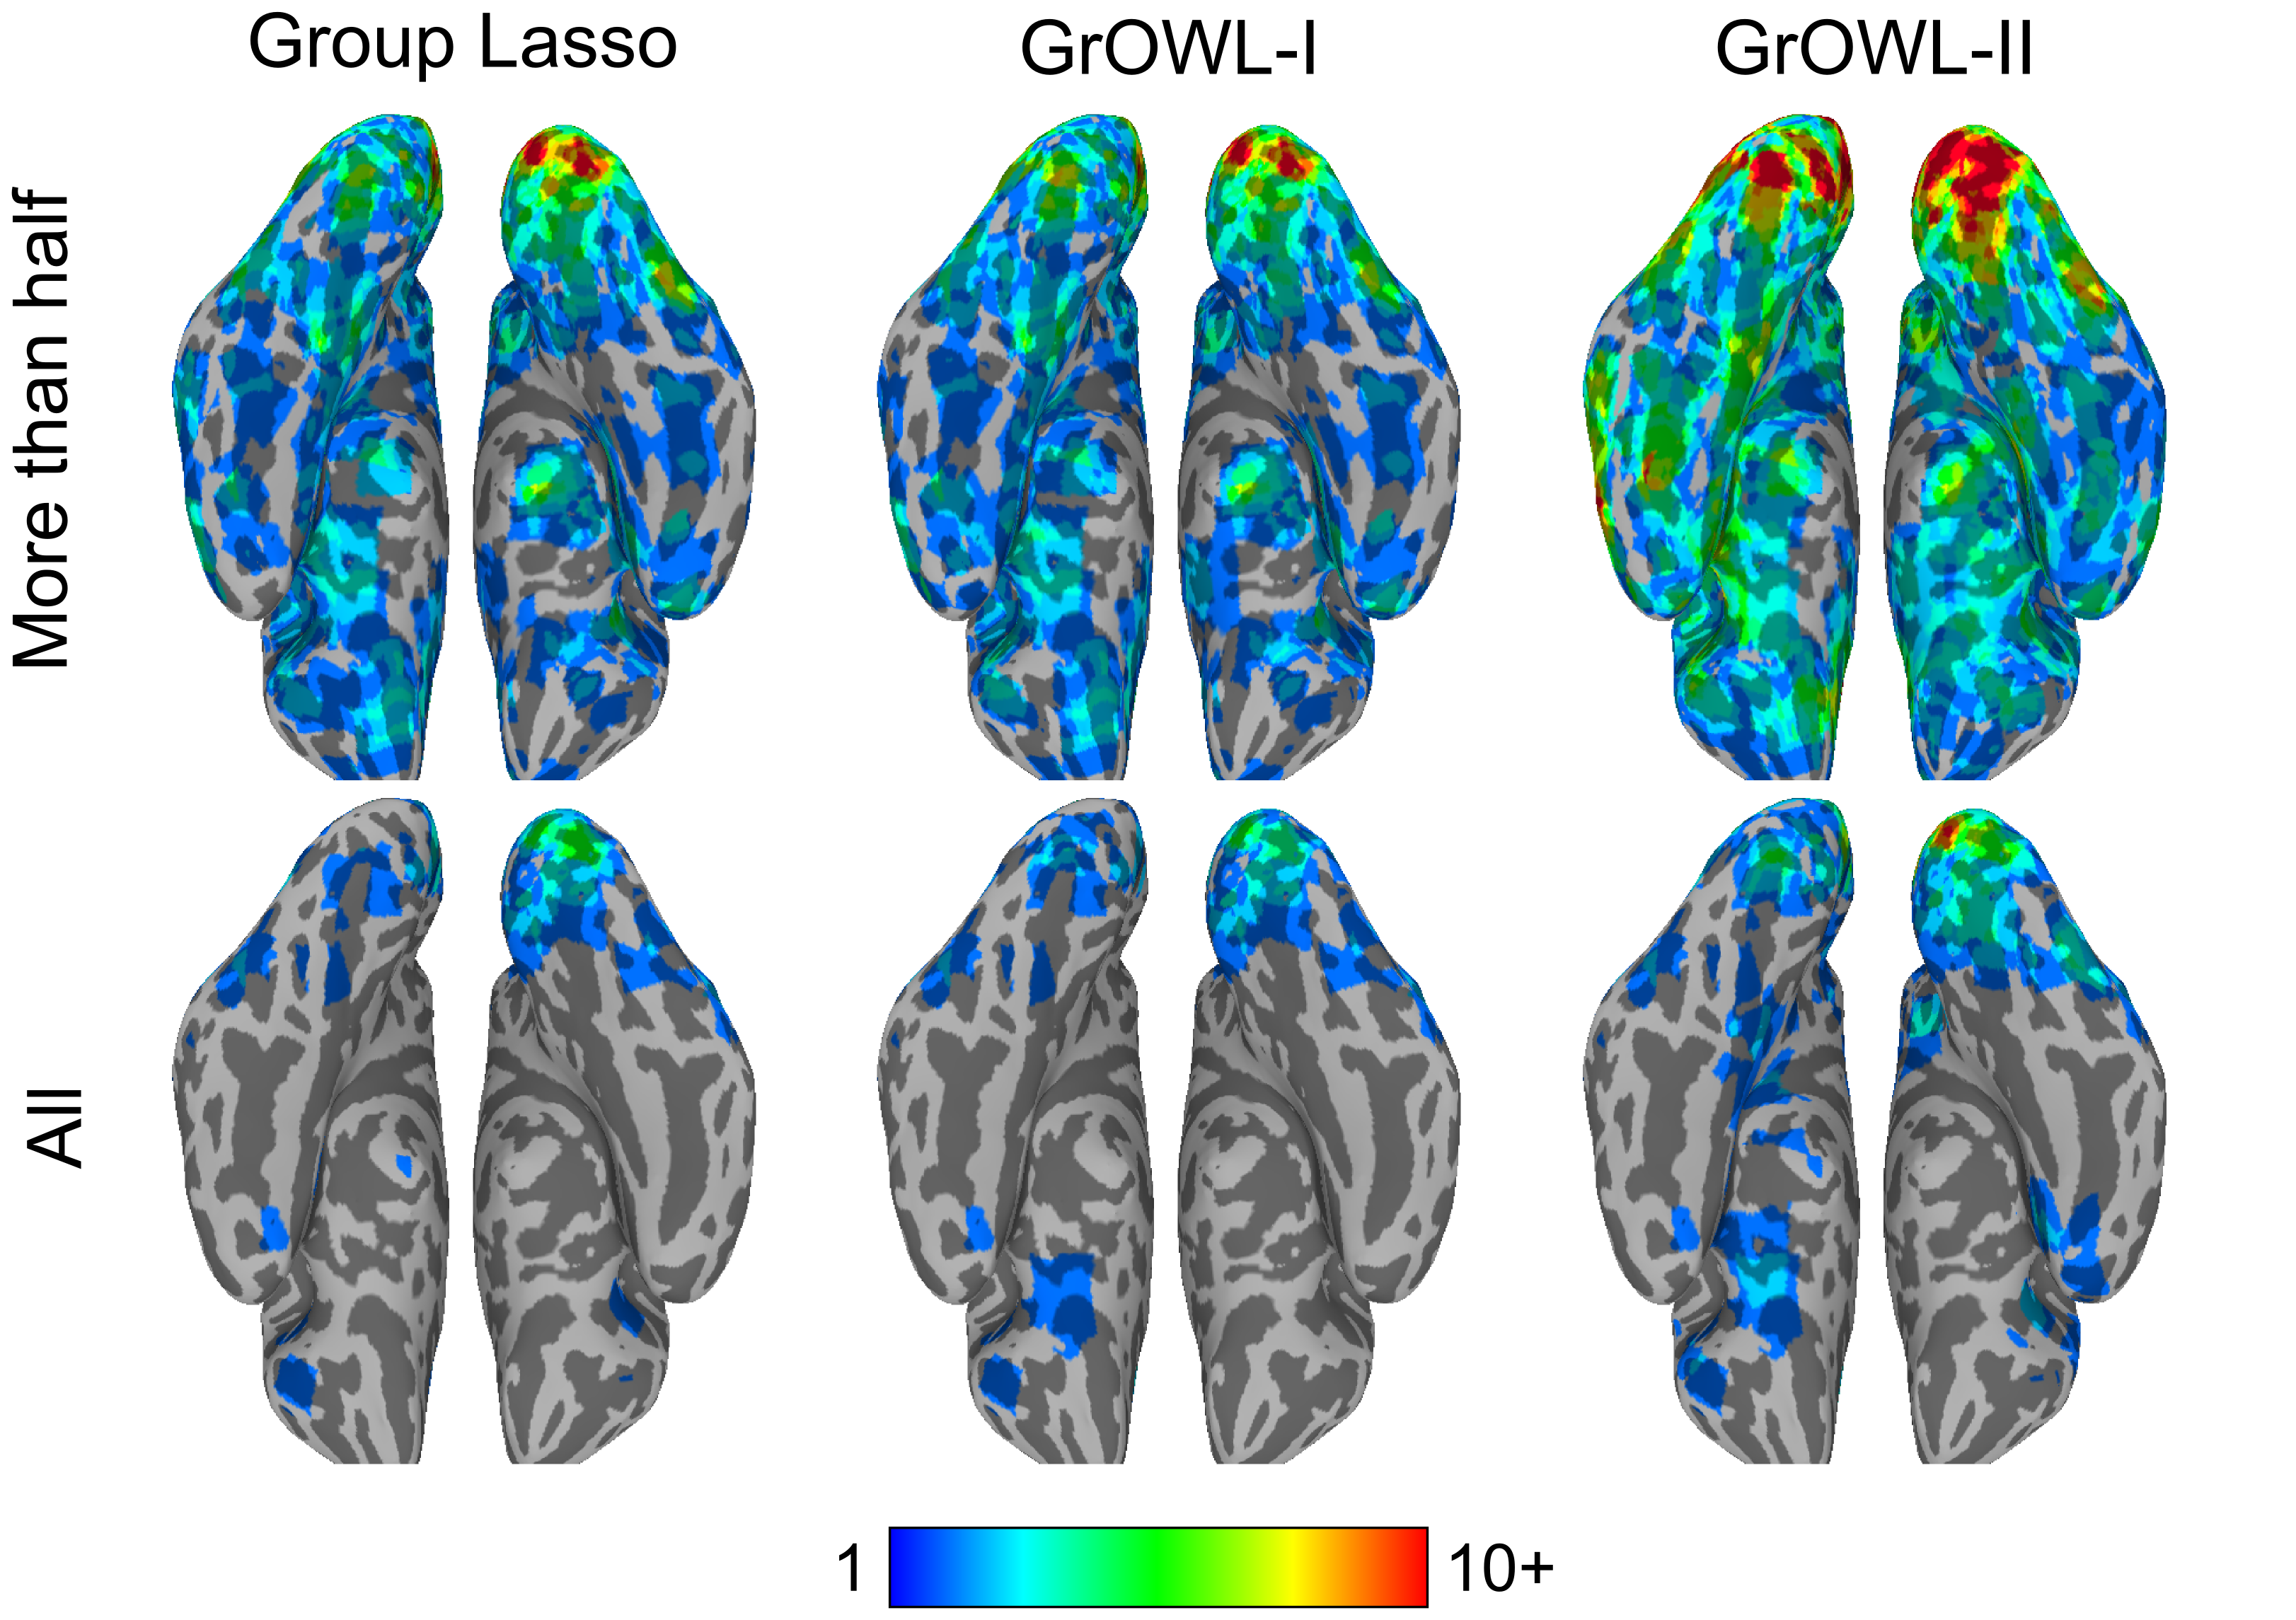
\includegraphics[width=0.75\textwidth]{brain_final.png}%
\caption{Brain plots.}
\label{fig.brain}
\end{figure*}

\begin{figure}[!t]
    \centering
  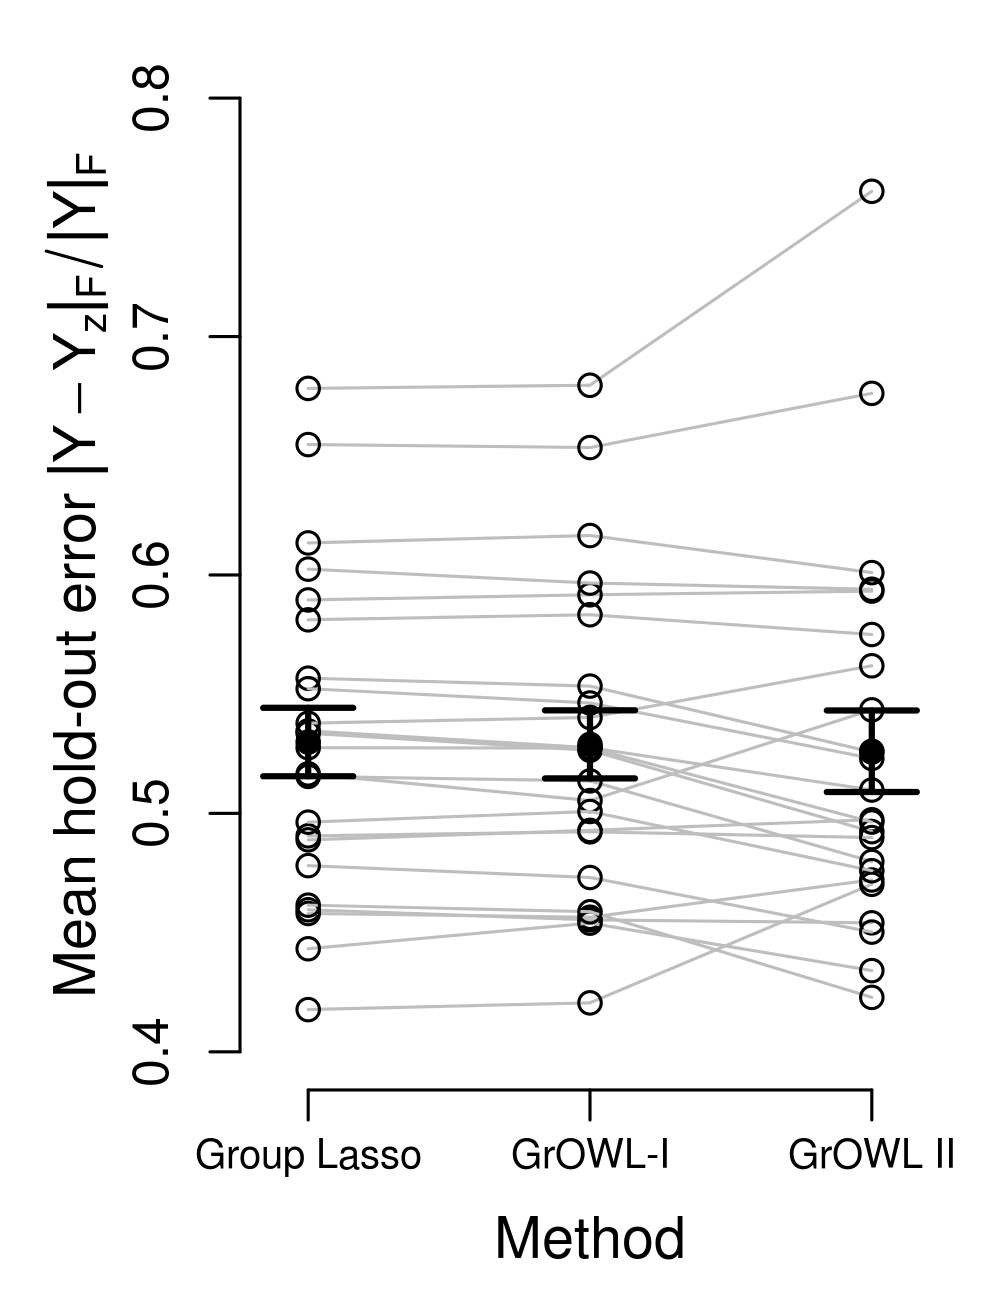
\includegraphics[width=0.35\textwidth]{Final_Error_Visual.png}
      
    \caption{Mean hold-out prediction error for group lasso and grOWLs with real data.}
    \label{fig.error}
  \end{figure}



\fi

